\section{Gilbert-Peierls' Algorithm}
Gilbert's Perierls \cite{GPAlgo} aimed for LU Decomposition of a matrix with partial pivoting with time proportional to the sum of floating-point operations, i.e., \bigo{flops(LU)}.The algorithm seems similar to the left-looking algorithm, although partial pivoting gives efficient traversing through the matrix. Following is the algorithm used.

\begin{algorithm}
    \caption{Gilbert-Peierls Algorithm: A Column-Oriented LU Factorization
        \label{algo:GP}}
    \begin{algorithmic}[1]
        \Require{$A$, a $n\times n$ asymmetric matrix}
        \Statex
        \State $L := I$
        \For{$j := 1 \textrm{ to } n$}
            \Comment{Compute $j^{th}$ column of $L$ and $U$}
            \State Solve $L_j u_j = a_j$ for $u_j$
            \State $b'_j := a'_j - L'j u_j$
            \State Do Partial Pivoting on $b'j$
            \State $u_{jj} := b_{jj}$
            \State $l'_j := b'_j / u_{jj}$
        \EndFor
    \end{algorithmic}
\end{algorithm}

\pagebreak

It computes $k^{th}$ column of $L$ and $U$ using previously computed $(k-1)^{th}$ columns of $L$ matrix. The notation used in the algorithm are as follows:
$j$ is the index of the column of $L$, and $U$ is computed in the $A$ matrix.Furthur $A$ matrix shared to $U$ as $a_j$ and $L$ as $a'_j$ as shown figure after going column $1$ to $N$ of $A$ matrix.

\begin{figure}[H]
    \centering
    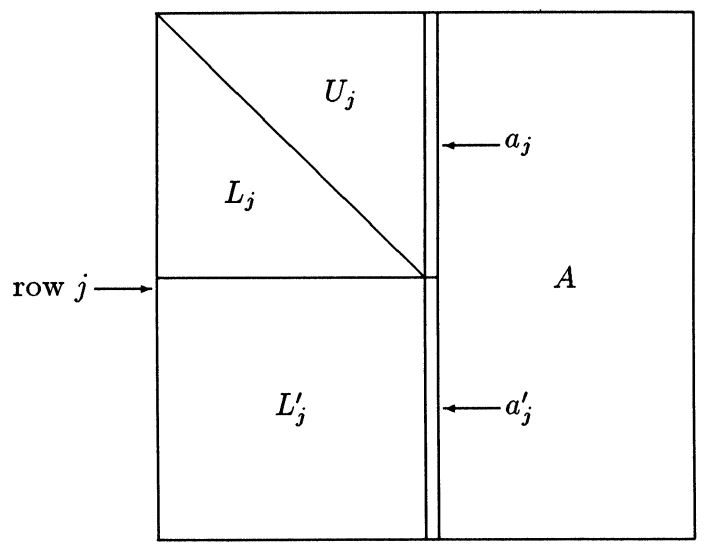
\includegraphics[width = 0.50\textwidth]{./Theory/gpConvention.JPG}
    \caption{Naming conventions used in algorithm}
    \label{fig:GP:namingConvention}
\end{figure}

State-of-the-art Gilbert-Peierl's algorithm \cite{GPAlgo} solve $Lx=b$ with \bigo{flops(LU)}.$Lx=b$ would iterate this for $N$ columns; therefore, the  \bigo{flops(LU)} is the efficiency of the algorithm.
This method requires locations of all non-zero elements in the sparse column vector x. The creation of a list of non-zero elements is referred in \textit{Symbolic Analysis}.

%\section{Symbolic Analysis}
% \label{sec:GP:symbolic}